\documentclass[main]{subfiles}
\begin{document}

%@@@@@@@@@@@@@@@@@@@@@@@@@@@@@@
% Main Topics: Passive Membrane Properties I - 11.10.2018
% Lecturer: Valerio Mante
% author: Vanessa Leite - base document from benelot/eth-intro-to-neuroinformatics-summary

\section{Passive (Cable) Membrane Properties}

\subsection{Biophysics of the membrane}
\begin{itemize}
\item Membrane separates in and out. It is an insulator/capacitor.
\item Ionic pumps: $[ion]_{in} \neq [ion]_{out}$
\item Selective ion channels
\end{itemize}

Those three factors give us the reversal (resting) potential: $E_{ion}$.

\subsection{Basic electronics}
\begin{itemize}[noitemsep,nolistsep]
	\item Ohm's Law: $V = I \cdot R$
	\item Kirchoff's Current Law (KCL): The sum of all currents entering and leaving any node in a circuit is zero.
	\item Kirchoff's Voltage Law (KVL): The sum of all voltages around a closed loop is equal to zero.
\end{itemize}

\subsection{Ion channel replacement circuit}
\begin{itemize}[noitemsep,nolistsep]
	\item Ion channel is equal to resistance.
	\item Ion gradient is equal to battery.
	\item Cell membrane is equal to capacitor.
	\item Conductivity $S=\frac{1}{R}$.
	\item Ion resistance is $R = V/I$.
	\item Ion conductivity is $\gamma = g_m = I/V$.
	\item Outward current for an ion is $I_m=g_m(V-E_m)$.
	\item If the concentration of an ion on one side is raised (with a corresponding molecule of opposite charge) and the membrane is permeable for this ion, then the side which has a higher concentration gets more negative, because the ions go to the other side, leaving behind uncompensated negative charges.
\end{itemize}
\begin{figure}[H]
	\centering
	\scalebox{0.7}{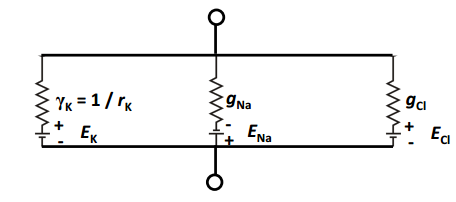
\includegraphics{ion_channel_circuit_01.png}}
\end{figure}
\begin{figure}[H]
	\centering
	\scalebox{0.7}{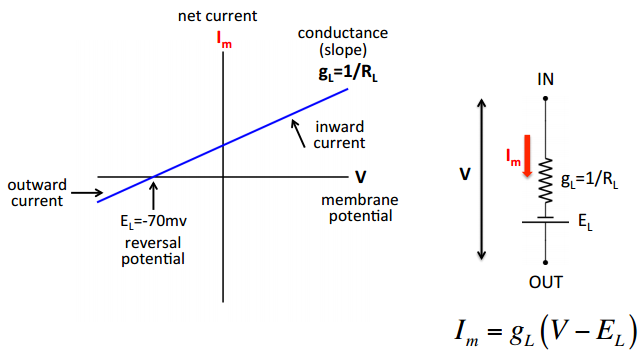
\includegraphics{current_voltage_01.png}}
\end{figure}

We say conductance is ohmic when we have passive properties, thus, $I = g \cdot V$.
Different channel types have different resting potential. For example, AMPA/NMDA (excitatory) have $E_{rev} \approx 0 mV$. GABA A and GABA B (inhibitory) have $E_{rev} \approx -65 mV$ and $-90 mV$, respectively.

Synapses are injecting (externeal) current.
Assume dendrite are passive cables that just conduct current (this is a simplification, we are discarding, for instance, backprop action potential and dendrite computation.). This way, we have three models:
\begin{itemize}
\item Single compartment model: voltage has only temporal dependency $V = V(t)$.
\item Cable equation: depends on time and location (analytical solutions) $V = V(x,t)$.
\item Multicompartment model: (numerical solutions) $V = V(x,t)$.
\end{itemize}

Those approaches offer a trade-of between realism and complexity.

\subsection{Single-compartment model}

\paragraph{Assumptions, configuration}
\begin{itemize}[noitemsep,nolistsep]
	\item Assume isopotential $V = V(t)$: holds locally
	\item Spherical membrane.
	\item $I_e$ is an injected current.
	\item $I_C$ is the capacitive current, charges the membrane.
	\item There is also a leak current $I_m = g_m(V-E_R)$.
	\item $[ion]_{in} = [ion]_{out} \rightarrow V_{rest} = 0$, equivalent to $v(t) = V(t) - E_R$
\end{itemize}

\paragraph{Membrane as electrical circuit}

At $t = 0$ an external current arrives, the membrane is charged and some current leak. At $t > 0$, $I_e > I_m$, i.e., the injected current is bigger than the leak current (some current is charging the membrane). At $t = \infty$,  we reach the equilibreium, $I_e = I_m$ and $I_C$ = 0, with the membrane completely charged, all the current that enters, leave.

\begin{itemize}[noitemsep,nolistsep]
	\item $I_e  - I_m = I_C$ and $I_m=g_m(V-E_R)$
	\item $C = \frac{Q}{V} \rightarrow CV = Q \rightarrow C\frac{dV}{dt} = \frac{dQ}{dt} = I_C$
	\item $I_e - gm \cdot v(t) = C_m \cdot \frac{dV(t)}{dt}$
	\item Membrane time-constant: $\tau_m = R_m \cdot C_m$
	\subitem depends on the resistances and the capacitors. Usual range from 10-100 ms.
	\item Larger current due to spatial summation.
	\item Less depolarization with small resistance (larger area).
\end{itemize}

\begin{figure}[H]
	\centering
	\begin{subfigure}[b]{0.3\textwidth}
		\centering
		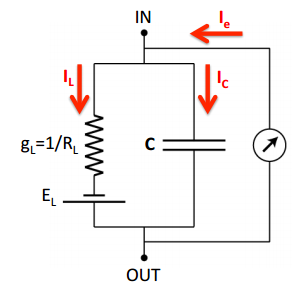
\includegraphics[width=\textwidth]{membrane_circuit_01.png}
	\end{subfigure}%
	~
	\begin{subfigure}[b]{0.5\textwidth}
		\centering
		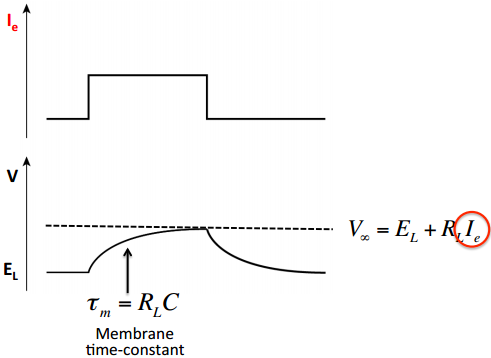
\includegraphics[width=\textwidth]{membrane_circuit_02.png}
	\end{subfigure}
	\caption{$R_L = R_m$, $E_L = E_m$, $g_L = g_m$, $I_L = I_m$}
\end{figure}

\subsubsection{Steady-state}
$R_m$ as input resistance.

$V_\infty = R_m \cdot I_e + E_m$: steady-state, i.e., voltage doesn't change anymore ($\frac{dV}{dt}=0$).

$V_\infty$ increases if $R_m$ increases (less leak) or $I_e$ increases (more input)

\paragraph{Consequences}
Two neurons with the same concentration of channels, differing only regarding the size: the smaller neuron will have more resistance, thus, for the same amount of current ($I_e$) it will have smaller voltage change ($R_{small neuron} \rightarrow V^{small}_\infty$ and $R_{large neuron} \rightarrow V^{large}_\infty$). Thus, $R_m = \frac{r_m}{area}$.

Two neurons, one myelinated and another unmyelinated. The myelinated has less resistance thus it needs less current input ($I_e$) to achieve the same voltage change.

\subsubsection{Time-dependency}
$\tau_m$ is the memory of cell $\approx 10$ to $100 ms$. Neuron forgets after $\tau$. Longer memory requires few mechanisms, for example, charge in synapse or recurrency.

\paragraph{several solutions}
\[V(t) = E_m + R_m \cdot I_e + (V(0) - E_m - R_m \cdot I_e) \epsilon^{\frac{-t}{\tau_m}}\]

\paragraph{single solution}
\[v(t) = v_\infty+(v(0)-v_\infty)e^{-\frac{t}{\tau_m}}\]
for $v = V - E_m$

\paragraph{Consequences}
Consider $I_{e1} \rightarrow V_1(t)$ and $I_{e2} \rightarrow V_2(t)$, then, $V_1(t) + V_2(t)$ is result of $I_{e1} + I_{e2}$.

\subparagraph{Spatial summation} 
Simultaneous inputs ($\delta t = 0$) sum linearly.
If $I_e \rightarrow k \cdot I_e$ then $V_\infty \rightarrow k \cdot V_\infty$.

\subparagraph{Sequential inputs}
Sequential inputs sum if $\delta t < \tau_m$.
It is quite fuzzy, very different from computers.

\subparagraph{Constant inputs}
When achieve the threshold, it generates an action potential and right after, reset it. This is knowing as Integrate and Fire neuron.
$r_{isi} = \frac{1}{t_{isi}} \approx \frac{E_m - V_{th} + R_m I_e}{\tau_m \cdot (V_{th} - V_{reset})}$

\subparagraph{idealized synapse}
if $I_e > 0$ then $V > E_m$ leading to EPSP (depolarization). 
if $I_e < 0$ then $V < E_m$ leading to IPSP (hyperpolarization).

\subsubsection{Equivalent electrical circuit}

\paragraph{Neuron}

\begin{figure}[H]
	\centering
	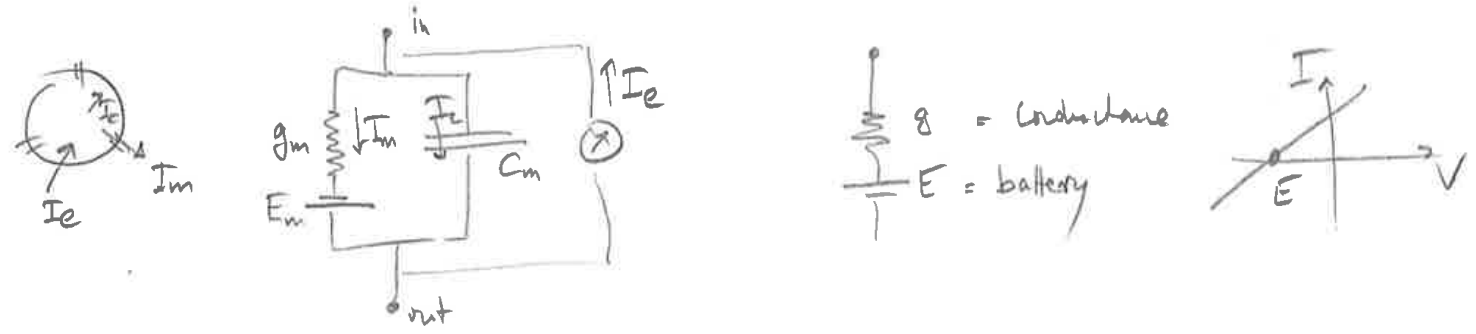
\includegraphics[width=\textwidth]{electrical_circuit_neuron.png}
	\caption{Equivalent electrical circuit for a neuron.}
\end{figure}

\paragraph{Adding synapse}

\begin{figure}[H]
	\centering
	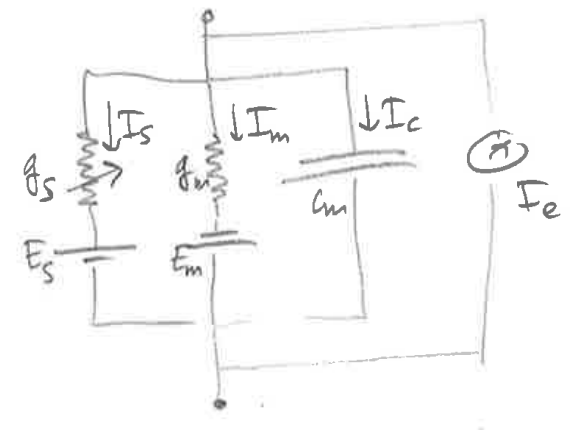
\includegraphics[width=0.5\textwidth]{electrical_circuit_neuron_synapse.png}
	\caption{Equivalent electrical circuit for a neuron including synapse. The conductance of a synapse ($g_s$) is variable and depends on presence of neurotransmitters.}
\end{figure}

$I_e = I_s + I_m + I_c \rightarrow I_e = C_m \frac{dV}{dt} + g_m (V - E_m) + g_s(V - E_s)$
In equilibrium $I_c = 0 \rightarrow I_e = g_s(V - E_s) + g_m (V - E_m) \rightarrow V_\infty = \frac{g_m \cdot E_m + g_s \cdot E_s + I_e}{g_m+g_s}$

\begin{itemize}[noitemsep,nolistsep]
	\item Equilibrium at $I_m=I_s$
	\item $V_\infty = \frac{g_m \cdot E_m + g_s \cdot E_s + I_e}{g_m+g_s}$
	\item For $g_s >> g_m$ (synapse open): $V_\infty = E_s + \frac{I_e}{g_s}$, thus the effect of $I_e$ is reduced: shunting inhibition ($V_{eq} \approx E_s$).
	\item For $g_s << g_m$ (synapse closed): $V_{eq} \approx E_m$.
%	\item $\tau_m = \frac{C}{g_L+g_S}$
\end{itemize}

\subsection{The cable equation}

So far, ions flow (in $\rightarrow$ out) to achieve $E_{rest}$. But, what if $V = V(t) \neq E_{rest}$ most of the time?

\paragraph{leak current}
$\sum_{time} I_{leak} \approx 0$: balance of exc. and inh, no action potential
\paragraph{synaptic current}
$\sum_{time} |I_s| > 0$: depletes concentration gradients $\rightarrow$ needs pump (needs energy).

\paragraph{Longitudinal current}

In the cable equation we use the same variables as before but we need to express $I_L$: longitudinal current. Now we have a current that flows inside the membrane (for instance, left to right).

\begin{figure}[H]
	\centering
	\scalebox{0.3}{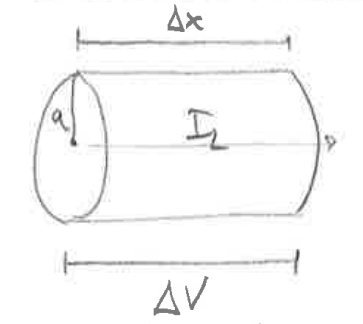
\includegraphics{longitudinal-current.png}}
	\caption{To start, let's consider a piece of cable of length $\delta x$. In this piece, we have a voltage drop $\Delta V$.}
\end{figure}

$R_L = \frac{r_L}{\pi a^2} \cdot \Delta x = \frac{r_L}{Area} \cdot \Delta x$.

\begin{itemize}
\item $r_L$ is a constant, a propertie of intracelullar medium.
\item $\frac{1}{Area}$: resistances in parallel $\rightarrow$ $\frac{1}{R_{total}} = \sum \frac{1}{R} \rightarrow R_{total} = \frac{R}{N}$.
\item $\Delta x$: in series $\rightarrow R_{total} = N \cdot R$
\end{itemize}

By Ohm's law: $\Delta V = R_L \cdot I_L = \frac{r_L}{\pi a^2} \Delta x I_L \rightarrow	(\Delta x \to 0) \frac{dV}{dx} x = - \frac{r_L}{\pi a^2} \cdot I_L(x)$. By definition, the sign is $-$: $\Delta V < 0$ for pos. current from $x \rightarrow dx + x$.

\paragraph{Charge conservation}

\begin{figure}[H]
	\centering
	\scalebox{0.3}{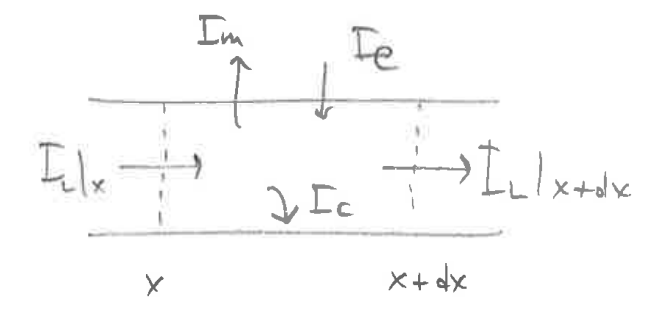
\includegraphics{charge-conservation.png}}
\end{figure}

In essence, $I_L(x + dx) = I_L(x) - I_m + I_e - I_c$, where:
\begin{itemize}
\item $I_c \approx \frac{\partial V}{\partial t}$
\item $I_m \approx gm (V - E_m)$
\item $I_L(x+dx) \approx \frac{\partial V}{\partial x}(x+dx)$
\end{itemize}

To derive cable equation:
\begin{itemize}
\item $I_m = 2 \pi a \cdot \Delta x \cdot i_m$
\item $I_e = 2 \pi a \cdot \Delta x \cdot i_e$
\subitem where $i_m$ and $i_e$ are current densities = current/Area
\item $I_L = \frac{\pi a^2}{r_L} \frac{\partial V}{\partial x}$
\item $I_c = 2 \pi a \Delta x C_m \frac{\partial V}{\partial t}$
\end{itemize}

\[c_m\frac{\partial V}{\partial t} = \frac{1}{2ar_L}\frac{\partial}{\partial x}(a^2\frac{\partial V}{\partial x})-i_m+i_e\]

\begin{figure}[H]
	\centering
	\scalebox{0.7}{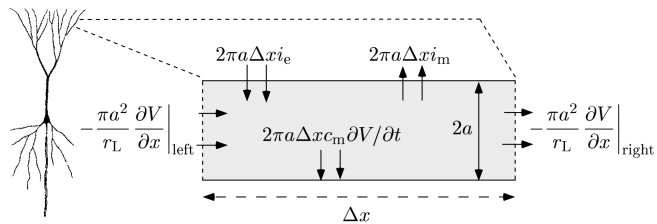
\includegraphics{cable_equation_01.png}}
\end{figure}

\paragraph{Note}
\begin{itemize}
\item $a$ need not to be continuous, i.e., $a = a(x)$.
\item $i_m$ could be very complicated
\item in general, there is no analytical solution
\subitem but we can consider simple cases where solution exists
\end{itemize}

Assume $a$ is continuous, $i_m = \frac{V - E_r}{r_m}$, and define $v = V - E_r$:

\[c_m\frac{\partial V}{\partial t} = \frac{a}{2r_L}\frac{\partial^2 v}{\partial x^2}- \frac{v}{r_m} + i_e\]


\paragraph{Define}
$\tau_m = r_m \cdot c_m$ (time constant) and $\lambda = \sqrt{\frac{a r_m}{2 r_L}}$ (length constant: "electrotonic length"), thus:

\[\tau_m\frac{\partial V}{\partial t} = \lambda^2 \frac{\partial^2 v}{\partial x^2} - v + r_m i_e\]

\subsubsection{Solution for simple cases}
%\begin{figure}[H]
%	\centering
%	\scalebox{0.7}{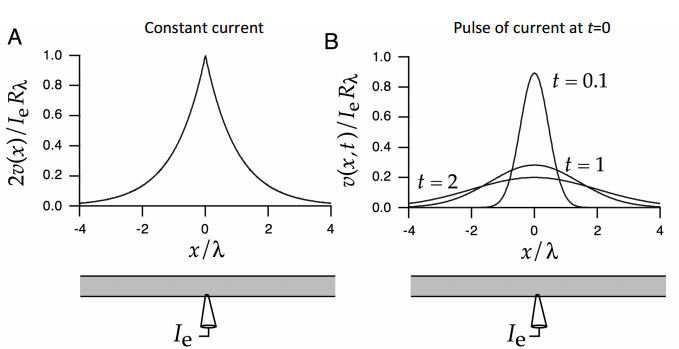
\includegraphics{cable_equation_02.png}}
%\end{figure}

\begin{figure}[H]
	\centering
	\begin{subfigure}[b]{0.6\textwidth}
		\centering
		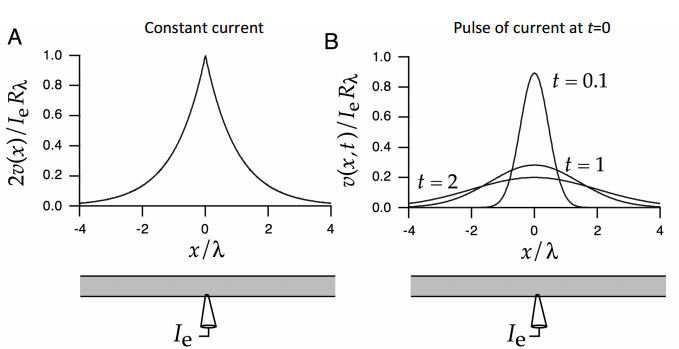
\includegraphics[width=\textwidth]{cable_equation_02.png}
	\end{subfigure}%
	~
	\begin{subfigure}[b]{0.3\textwidth}
		\centering
		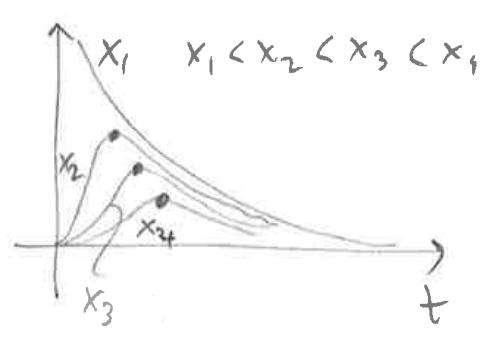
\includegraphics[width=\textwidth]{cable-equation-t.png}
	\end{subfigure}
	\caption{Left: constant current by location; center: pulse of current by location; right: pulse of current by time.}
	\label{fig:cable-equation}
\end{figure}

\paragraph{Infinite cable, constant $I_e$ (not time varying) and steady state solution $V=V(x)$ for $t \to \infty$}
for $\frac{\partial V}{\partial t} = 0 \rightarrow V_\infty (x) = \frac{I_e R_\lambda}{2}\exp(-\frac{|x|}{\lambda})$

\subparagraph{Consequences}
\begin{itemize}
\item  If $I_e$ injected at $x = 0$ in dendrite (e.g., through synapse)
\subitem $V(x)$ decays exponentially with distance
\subitem $V(x)$ reduced to $\frac{1}{e}$ at $x = \lambda$ compared to $V(x = 0)$
\item dendrites have effective length close to $\lambda$ (or in that order of magnitude)
\subitem strong alternation of $V(x)$ from distal dendrites to soma.
\item increase in $\lambda$:
\subitem $r_m$ increases: less leak current $I_m$
\subitem $r_L$ decreases: less intracelullar resistance
\subitem $a$ increases: larger cable
\end{itemize}

\paragraph{Finite cable - dendrites}
length of the cable decreases $\rightarrow$ closer to isopotential.

\paragraph{Infinite cable, pulse of input current ($I_e = \delta x \delta t$)}
At each time $t$, $V(x,t)$ is a gaussian in $x$.
The width of the gaussian is $r  = \lambda \sqrt{\frac{t}{\tau_m}}$, where $\lambda$ is a spatial scale and $\tau_m$ is a temporal scale.
The area of the gaussian is given approximately by $e^\frac{-t}{\tau_m}$. The area decrease with time, some charge is lost through $i_m$.

Ploting $V$ as a function of time (~\ref{fig:cable-equation}) for different $x$:
\begin{itemize}
\item time of max $V$ changes with $x$
\item width of peak changes with $x$
\item by looking at the peak and the time occurrence of the peak at the soma one can infer about how far from the dendrite the current was injected.
\item "speed" of the bump: $V_{bump} \approx 2 \cdot \frac{\lambda}{\tau_m}$.
\subitem this approximation also holds for action potentials: $V_{ap} \approx 0.25 -100 mV$
\subitem if $\lambda$ increases, $V$ goes far, thus $V_{bump}$ increases
\subitem if $\tau_m$ increases, $V$ changes slowly, thus $V_{bump}$ decreases
\end{itemize}

How to increase $V_{bump}$?
\begin{itemize}
\item by increasing $a$: giant axon
\item myelin: $r_m$ increases and $c_m$ decreases.
\end{itemize}

$V_{bump} = \sqrt{\frac{1}{2 r_m r_L}} \frac{1}{c_m}$

\begin{itemize}[noitemsep,nolistsep]
	\item $v(x) = \frac{I_eR_\lambda}{2}\exp(-\frac{|x|}{\lambda})$
	\item $R_\lambda=\frac{r_m}{2\pi a\lambda} = \frac{r_L\lambda}{\pi a^2}$
	\item $\lambda = \sqrt{\frac{ar_m}{2r_L}}$ sets the scale for the spatial variation in the membrane potential.
	\item $\lambda$ is the electronic length, or how far the signal travels.
	\item $\tau_m = r_mc_m$ sets the scale for the temporal variation in the membrane potential.
	\item $v(x,t) = \frac{I_eR_\lambda}{\sqrt{4\pi\lambda^2t/\tau_m}}\exp(-\frac{\tau_mx^2}{4\lambda^2t})\exp(-\frac{t}{\tau_m})$
	\item $a$ is the radius of the axon, about $2\,\mu m$
	\item $r_m$ is the specific membrane resistance, about $1\,M\Omega\cdot mm^2$
	\item $v = V - V_{rest}$
	\item $r_L$ is the longitudinal resistance, about $1\,k\Omega\cdot mm$
	\item $I_e$ is the injected current.
	\item It follows, that increasing $R_m$ also increases $\lambda$. With better isolation, signals travel further.
	\item Increasing the diameter also increases $\lambda$.
\end{itemize}

\subsection{Level of approximation}
\begin{itemize}[noitemsep,nolistsep]
	\item A neuron can be represented by a variable number of discrete compartments.
	\item Compartments represent a region, each with a single membrane potential.
	\item The connections between compartments have resistive couplings.
	\item The basic model is the single compartment (isopotential)
	\item There is also a model for selective ion channels: drive $V$ towards reversal potential ($E$) for that channel type
\end{itemize}

\end{document}
